\documentclass[10pt,twocolumn,letterpaper]{article}

\usepackage{cvpr}
\usepackage{times}
\usepackage{epsfig}
\usepackage{graphicx}
\usepackage{amsmath}
\usepackage{amssymb}

% Include other packages here, before hyperref.

% If you comment hyperref and then uncomment it, you should delete
% egpaper.aux before re-running latex.  (Or just hit 'q' on the first latex
% run, let it finish, and you should be clear).
\usepackage[breaklinks=true,bookmarks=false]{hyperref}

\cvprfinalcopy % *** Uncomment this line for the final submission

%\def\cvprPaperID{****} % *** Enter the CVPR Paper ID here
%\def\httilde{\mbox{\tt\raisebox{-.5ex}{\symbol{126}}}}

% Pages are numbered in submission mode, and unnumbered in camera-ready
%\ifcvprfinal\pagestyle{empty}\fi
\setcounter{page}{1}
\begin{document}

%%%%%%%%% TITLE
\title{Emotion from music spectrograms}

\author{Matteo Cerutti\\
Politecnico di Torino\\
{\tt\small s265476@studenti.polito.it}
% For a paper whose authors are all at the same institution,
% omit the following lines up until the closing ``}''.
% Additional authors and addresses can be added with ``\and'',
% just like the second author.
% To save space, use either the email address or home page, not both
\and
Antonio Santoro\\
Politecnico di Torino\\
{\tt\small s264014@studenti.polito.it}
\and
Marco Testa\\
Politecnico di Torino\\
{\tt\small s265861@studenti.polito.it}
}


\maketitle
%\thispagestyle{empty}

%%%%%%%%% ABSTRACT
\begin{abstract}
   
\end{abstract}

%%%%%%%%% BODY TEXT
\section{Introduction}

Nowadays people need to have the possibility to select music and make playlists based on their mood. Many music platforms feature different music playlists made by hand that include popular and commercial songs aiming to maximise ratings. One of the most used feature on these platforms is to create playlists similar to other ones, the point is that all the songs that will be included are selected on the "similarity". 
Since the intention was to stay inside the computer vision domain, we have to treat audio files as images so the first idea was to exploit spectrograms. After some researches, we found that our idea was applied to classify song genres, therefore starting from the article of Piotr Kozakowski and Bartosz Michalak \cite{Kozakowski}, we adapted their work to our objective.
The interest is to train a neural network on different audio speeches that represent different human emotions, extract features and try to see whatever those peculiarities can be matched from music. Amiriparian \etal \cite{Amiriparian} showed that processing spectrograms into networks characterized by a different depth the result will change. This report presents results obtained from three networks, ResNet152, VGG11 and GoogLeNet, trained on the RAVDESS Emotional song audio dataset \cite{Ravdess} and tested on the CAL500 dataset \cite{CAL500}.

\section{Data preparation}

\subsection{Training dataset}

The RAVDESS Emotional song audio consists of 1012 files of actors singing four seconds in a neutral North American accent. The portion used for this work includes calm, happy, sad, angry, and fearful emotions, each vocal is produced at two levels of emotional intensity, normal and strong.

Files are provided as .wav (16bit, 48kHz) that need to be converted into a raw spectrogram. For the purpose "SoX (Sound eXchange) sound processing utilities" has been used. This tool can process audio files and do things like trimming or filters frequencies. Spectrograms for the training dataset have been generated to fit the input size of the three networks, furthermore, to cope with the limited size of the dataset, augmentation has been applied like random grey colorizing, brightness, contrast and hue variations. Amiriparian \etal \cite{Amiriparian} showed that using different shade of colour could exhibit different outcomes but, since the hue transformation made by the PyTorch framework has a not negligible impact on the brightness of the image and the goal is to not alter any information on the spectrogram, the best choice was to stick with the original shades, hence playing with the contrast and with a monochrome image could have a positive effect on capturing some features.

\subsection{Test dataset}



\section{Training phase}

\section{Testing}

\section{Conclusions}


\begin{figure}[t]
\begin{center}
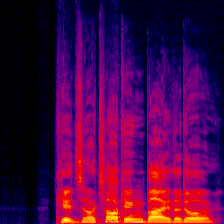
\includegraphics[width=0.8\linewidth]{img/happy_92.png}
\end{center}
   \caption{Training spectrogram sample.}
\label{fig:training_sample}
\end{figure}

\subsection{Miscellaneous}

\noindent
Compare the following:\\
\begin{tabular}{ll}
 \verb'$conf_a$' &  $conf_a$ \\
 \verb'$\mathit{conf}_a$' & $\mathit{conf}_a$
\end{tabular}\\
See The \TeX book, p165.

The space after \eg, meaning ``for example'', should not be a
sentence-ending space. So \eg is correct, {\em e.g.} is not.  The provided
\verb'\eg' macro takes care of this.


\begin{figure*}
\begin{center}
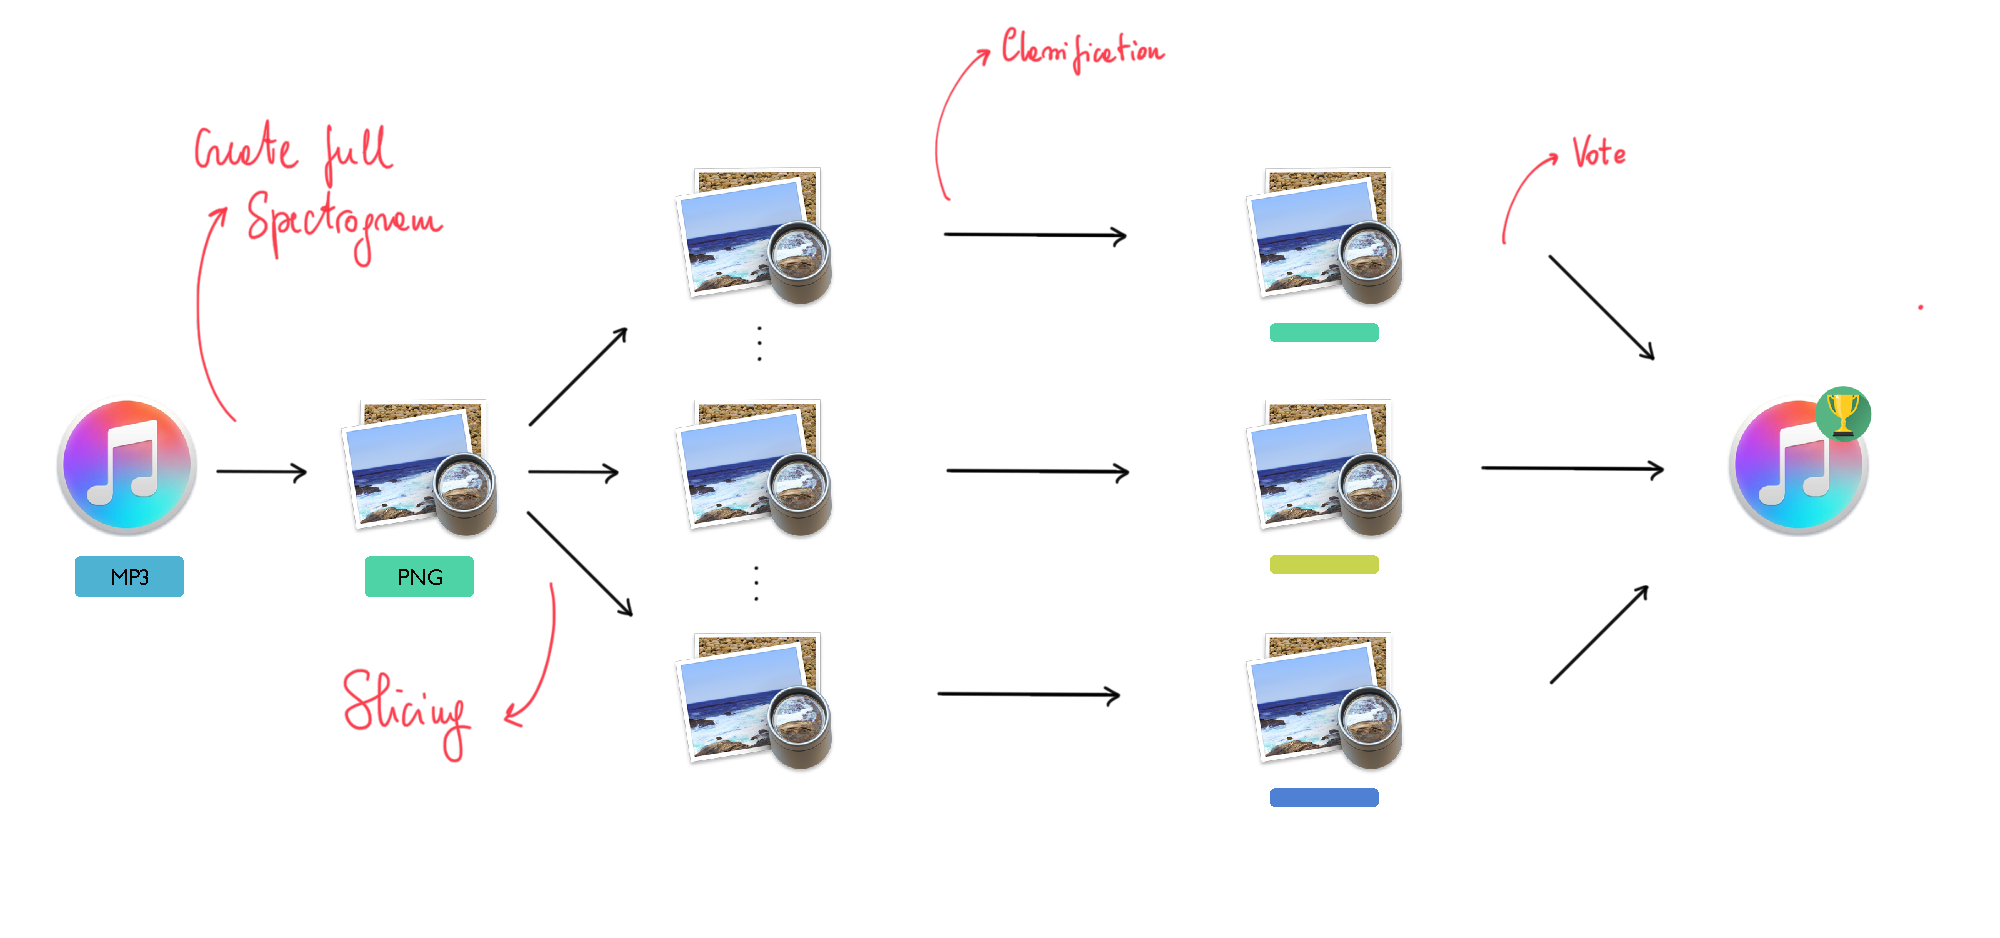
\includegraphics[width=0.8\linewidth]{img/Pipeline-project}
\end{center}
   \caption{Classification pipeline.}
\label{fig:pipeline}
\end{figure*}


\subsection{Footnotes}

Please use footnotes\footnote {This is what a footnote looks like.  It
often distracts the reader from the main flow of the argument.} sparingly.
Indeed, try to avoid footnotes altogether and include necessary peripheral
observations in
the text (within parentheses, if you prefer, as in this sentence).  If you
wish to use a footnote, place it at the bottom of the column on the page on
which it is referenced. Use Times 8-point type, single-spaced.


\begin{table}
\begin{center}
\begin{tabular}{|l|c|}
\hline
Method & Frobnability \\
\hline\hline
Theirs & Frumpy \\
Yours & Frobbly \\
Ours & Makes one's heart Frob\\
\hline
\end{tabular}
\end{center}
\caption{Results.   Ours is better.}
\end{table}

\subsection{Illustrations, graphs, and photographs}

All graphics should be centered.  Please ensure that any point you wish to
make is resolvable in a printed copy of the paper.  Resize fonts in figures
to match the font in the body text, and choose line widths which render
effectively in print.  Many readers (and reviewers), even of an electronic
copy, will choose to print your paper in order to read it.  You cannot
insist that they do otherwise, and therefore must not assume that they can
zoom in to see tiny details on a graphic.

When placing figures in \LaTeX, it's almost always best to use
\verb+\includegraphics+, and to specify the  figure width as a multiple of
the line width as in the example below
{\small\begin{verbatim}
   \usepackage[dvips]{graphicx} ...
   \includegraphics[width=0.8\linewidth]
                   {myfile.eps}
\end{verbatim}
}

{\small
\bibliographystyle{ieee_fullname}
\bibliography{egbib}
}


\end{document}
